% --------------------------
% ---- DECLARE PACKAGES ----
% --------------------------
\documentclass[a4paper, oneside, openright]{book}
\usepackage[T1]{fontenc} % Font encoding, T1 = it
\usepackage{lmodern}
\usepackage{booktabs}
\usepackage{multicol} % Per il frontespizio
\usepackage[utf8]{inputenc} % Input encoding - per caratteri particolari
\usepackage[english]{babel} % Lingua principale italiano, con parti in inglese
\usepackage{blindtext} % Per la generazione di paragrafi lorem ipsum
\usepackage{graphicx} % Per includere immagini esterne
\usepackage[a4paper,top=2.5cm,bottom=2.5cm,left=3cm,right=3cm]{geometry} %impaginazione e margini documento
\usepackage[fontsize=13pt]{scrextend} %dimensione font
\usepackage{graphicx}
\usepackage[parfill]{parskip} % Disabilita l'indentazione dopo essere andati a capo
% \usepackage[hang,flushmargin]{footmisc} % Disabilita l'indentazione nelle footnotes
\usepackage{titlesec}
\usepackage{minted} % Per i blocchi di codice
\usepackage{float}
\usepackage{amsmath} % For advanced math typesetting
\usepackage{amssymb} % For additional symbols, if needed
\usepackage{graphicx} % For including figures, if applicable
\usepackage[font=scriptsize, skip=5pt]{caption} % Spazio tra la caption e l'immagine
\usepackage[backend=biber, style=numeric, backref=true,defernumbers=true]{biblatex}
\usepackage[immediate]{silence}
\WarningFilter[temp]{latex}{Command} % silence the warning
\usepackage{sectsty}
\DeactivateWarningFilters[temp] % So nothing unrelated gets silenced
\usepackage{hyperref} % Rende l'indice cliccabile
\usepackage[justification=centering]{caption} % Per centrare le captions
\usepackage{csquotes} % Dipendenza di babel
\usepackage[bottom]{footmisc} % Posiziona le footnotes alla fine della pagina
\usepackage{hyperref}
\usepackage{enumitem}
\usepackage{amsmath, amssymb, graphicx}
\usepackage{hyperref}
\newcommand{\cmark}{\ding{51}}  % checkmark
\newcommand{\xmark}{\ding{55}}  % x-mark
\usepackage{pifont}

% ------------------------
% ---- DOCUMENT SETUP ----
% ------------------------
\pagestyle{plain}
\raggedbottom % Se la pagina non è completa, lascia lo spazio alla fine

\titleformat{\chapter}[display]
    {\normalfont\huge\bfseries}{}{0pt}{\LARGE} % Remove chapter number display
\titlespacing*{\chapter}{0pt}{0pt}{20pt} 
\chaptertitlefont{\fontsize{22pt}{30pt}\selectfont}

\hypersetup{ % Setup dell'aspetto dei link
    colorlinks,
    citecolor=black,
    filecolor=black,
    linkcolor=black,
    urlcolor=black
}

% \renewcommand{\footnoterule}{ % Rende la linea delle footnotes larga tutta la pagina
%   \kern -3pt
%   \hrule width \textwidth height 1pt
%   \kern 2pt
% } 
\renewcommand{\footnotesize}{\fontsize{11pt}{13pt}\selectfont} % Imposta la dimensione del testo delle footnotes
\setlength{\footnotesep}{0.5cm} % Imposta lo spazio fra e singole footnotes
\setlength{\skip\footins}{1.5cm} % Imposta lo spazio fra il corpo e le footnotes

\DeclareUnicodeCharacter{02BC}{}

% ------------------------
% ---- DOCUMENT START ----
% ------------------------
\addbibresource{bibliography.bib} % Importiamo la bibliografia
\begin{document} % Inizio documento
\pagenumbering{gobble} % Disabilita numerazione pagine
\begin{titlepage}
\begin{figure}[!htb]
    \centering
    
\includegraphics[width=8cm]{Images/Logo_Politecnico_Milano.png}
\end{figure}

\begin{center}
    \LARGE{\textbf{POLITECNICO DI MILANO}} \\[2mm]
    
    \small{\textbf{MASTER'S PROGRAM IN}} \\[1mm]
    
    \small{\textbf{HIGH PERFORMANCE COMPUTING ENGINEERING}} \\[2mm]
\end{center}

\vspace*{\fill}

\begin{center}
    \Large{\textbf{Software Engineering for HPC}}\\
\Large{\textbf{SustainCity Project}}
\end{center}

\vspace*{\fill}

\begin{minipage}[t]{1\textwidth}
    \vspace{-10mm}
    {\small \textbf{Group Members:}}\\[2mm]
    {\small
    Salvatore Mariano Librici \hfill Person Code: 11078653\\
    Rong Huang \hfill Person Code: 10948935\\
    Yibo Li \hfill Person Code: 11022291\\
    Zhaochen Qiao \hfill Person Code: 11021721\\
    }
\end{minipage}



\vspace{10mm}

\begin{center}
    {\small{\textbf{Academic Year:}}{\small\vspace{0.5mm}
    \\ \small{2024/2025}}}  
\end{center}

\end{titlepage}
 % PAGINA FRONTESPIZIO

\pagenumbering{arabic} % Riabilita la numerazione in modo che cominci dal primo capitolo
\setcounter{chapter}{0} % Fa risultare l'introduzione come capitolo 0
% ------------------
% ---- CHAPTERS ----
% ------------------
\newpage
\begin{titlepage}
\centering

\vspace*{2cm}

% LOGO

\includegraphics[width=0.35\textwidth]{Images/UrbanLeaf.jpeg} \\[1.5cm]

% TITLE
{\Huge \textbf{UrbanLeaf}}\\[0.5cm]
{\large Smart Urban Mobility Management System} \\[1cm]

% SHORT DESCRIPTION
\parbox{0.85\textwidth}{
\centering
UrbanLeaf is a software solution designed to enhance urban sustainability through intelligent traffic management and event-aware mobility planning.\\[1mm]
By leveraging real-time data, historical patterns, and event forecasts, UrbanLeaf supports both automated decisions and human oversight in city-wide transport optimization.
}

\vfill

{\small Project Code: \texttt{SustainCity} \hspace{1cm} Version: 1.0 \hspace{1cm} April 2025}

\end{titlepage}


\tableofcontents  % Genera l'indice


\newpage
\chapter{The Project and Project Goals}

\subsection{Overview}

The UrbanLeaf project aims to tackle pressing global issues such as climate change and environmental sustainability, which are significantly impacted by urban transportation systems. In particular, the project focuses on reducing the negative effects of city commuting by leveraging data-driven technologies and adaptive control mechanisms.

This project is part of the Software Engineering for HPC course and is designed to apply the principles of requirement engineering and architectural design learned in the first part of the course.

\subsection{Project Goals}

The system to be designed will analyze urban traffic conditions and apply or suggest actions that optimize transportation infrastructure. The goals are divided into three categories:

\begin{itemize}
    \item \textbf{Type 1 – Real-Time Traffic Light Adjustment:} Dynamically modify the duration of green and red lights at intersections based on live traffic conditions collected via road sensors.
    
    \item \textbf{Type 2 – Pattern-Based Optimization:} Analyze recurring traffic patterns to suggest optimizations such as changing road directions (e.g., one-way), traffic light configurations, and public transport schedules.
    
    \item \textbf{Type 3 – Event-Based Planning:} Collect information about planned large-scale public events and generate event-specific transportation plans. This includes changes in public transport, traffic light behavior, and road accessibility.
\end{itemize}

\subsection{Technical Context}

The system will integrate with several existing data sources:
\begin{itemize}
    \item An event-based sensor infrastructure that tracks vehicle crossing times at intersections.
    \item A microservice providing public transport schedules, with API support for querying by street or line.
    \item A news feed or event channel that provides early notifications of upcoming events.
\end{itemize}

\subsection{Reporting and Logging}

The system must also:
\begin{itemize}
    \item Automatically log all actions taken under Type 1.
    \item Generate daily public reports with traffic flow data and Type 1 actions.
    \item Generate yearly reports outlining all Type 2 and Type 3 suggestions, indicating whether they were accepted or rejected by city managers.
\end{itemize}


\newpage
\chapter{Requirement Analysis}

\subsection{Relevant Human and Non-Human Actors}

\textbf{Human Actors:}
\begin{itemize}
    \item \textbf{Traffic Managers} – Access daily reports (Type 1), review and approve/reject optimization proposals (Type 2 and Type 3).
    \item \textbf{Citizens} – Receive real-time traffic data (Type 1), and event-based routing suggestions (Type 2, 3) through the application.
    
    \item \textbf{Event Organizers} – Submit data about upcoming public events (Type 3).
\end{itemize}



\textbf{Non-Human Actors:}
\begin{itemize}
    \item \textbf{Sensor System} – Event-based system that provides real-time traffic flow data (Type 1).
    \item \textbf{Public Transport Microservice} – Provides public transportation timetables (Type 2, Type 3).
    \item \textbf{Public Transport Schedulers} – Provide bus/tram schedules in response to accepted system recommendations (Type 2 and 3).
    \item \textbf{Traffic Light System} – Accepts dynamic configuration changes (Type 1 and 3).
    \item \textbf{News Channel} – Publishes upcoming events (Type 3).
    
\end{itemize}

\newpage
\subsection{Use Cases}

This section describes the main use cases of the UrbanLeaf System. The use cases model the interactions between external actors (citizens, managers, event organizers, sensors, and other systems) and the functionalities provided by the application. These interactions are visualized in the use case diagram below.

\vspace{1em}
\begin{center}
    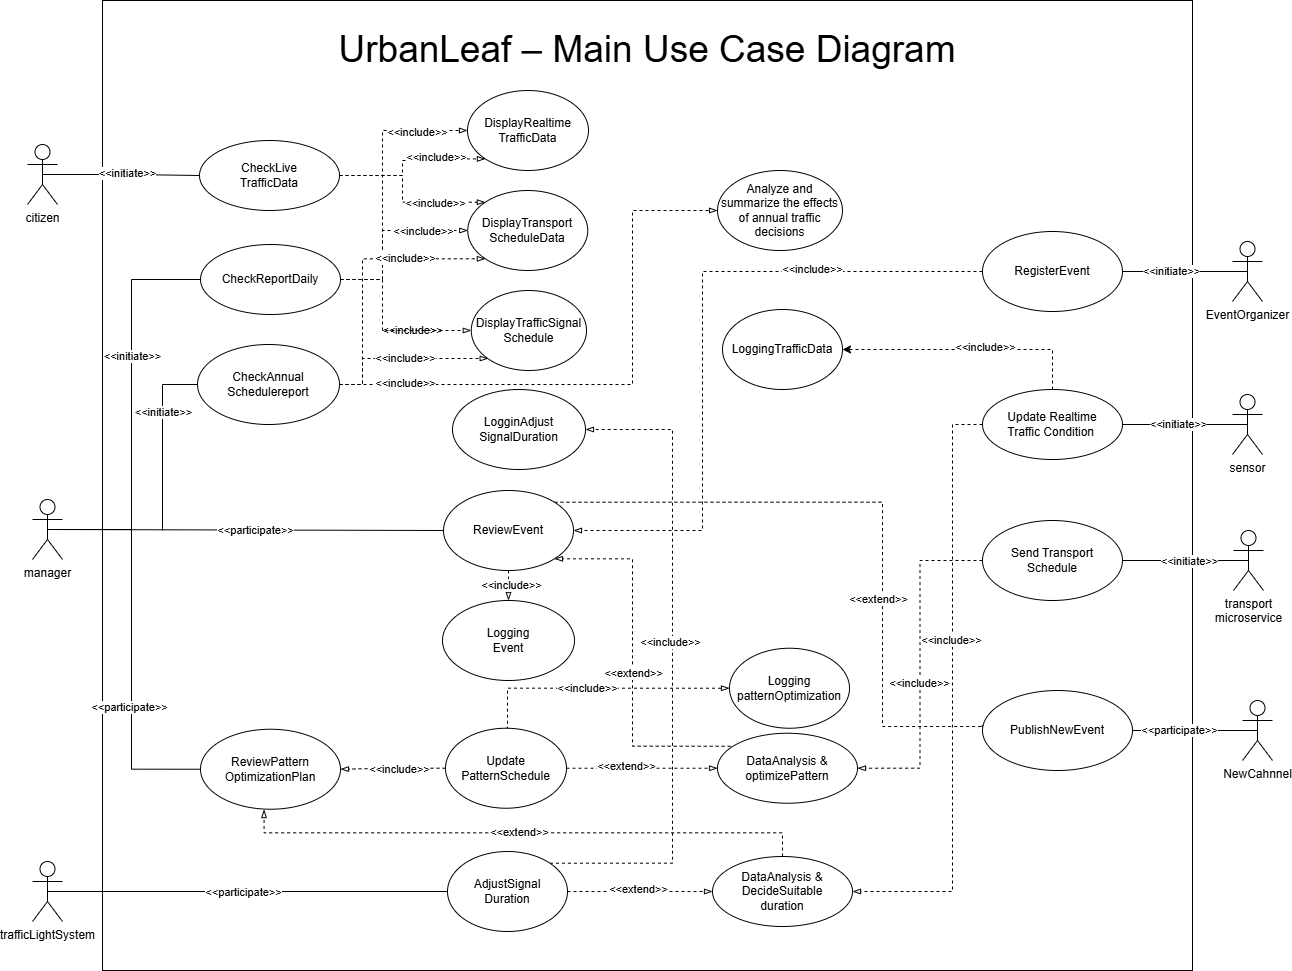
\includegraphics[width=1\textwidth]{Images/UseCase.png}
\end{center}
\vspace{1em}

\subsubsection*{Overview of Represented Use Cases}

\begin{itemize}
    \item \textbf{CheckLiveTrafficData}: Citizens access real-time traffic information through the app. This use case includes:
    \begin{itemize}
        \item \textit{DisplayRealtimeTrafficData}
        \item \textit{DisplayTransportScheduleData}
        \item \textit{DisplayTrafficSignalSchedule}
    \end{itemize}

    \item \textbf{CheckReportDaily / CheckAnnualScheduleReport}: Managers view daily and yearly traffic-related reports. The annual report includes system decisions and long-term insights.

    \item \textbf{RegisterEvent}: Event organizers register upcoming public events, including location, time, and estimated attendance.

    \item \textbf{UpdateRealtimeTrafficCondition}: The sensor system sends continuous real-time traffic flow data to the application.

    \item \textbf{SendTransportSchedule}: The public transport microservice provides schedules for buses and trams, which are used by the system to plan responses.

    \item \textbf{ReviewEvent / ReviewPatternOptimizationPlan}: Traffic managers access the dashboard to review system-generated suggestions related to events or recurring traffic patterns.

    \item \textbf{UpdatePatternSchedule / AdjustSignalDuration}: Once suggestions are approved by managers, the system updates transport schedules or modifies signal timing accordingly.

    \item \textbf{PublishNewEvent}: The News Channel actor receives and publishes relevant traffic and event information for public visibility.

    \item \textbf{LoggingTrafficData, LoggingEvent, LoggingPatternOptimization}: All key actions are recorded for traceability, report generation, and audit purposes.
\end{itemize}

\subsubsection*{Additional Use Cases (Not Represented in Diagram)}

In addition to the diagrammed use cases, the following functionalities are part of the system's behavior:

\begin{itemize}
    \item \textbf{Notify Rerouting Information to Citizens (T1, T3)}: Citizens receive personalized routing suggestions in case of detected congestion or planned events.

    \item \textbf{Handle System Errors and Log Failures (All)}: The system monitors component interactions and logs any data or service-related failures.

    \item \textbf{Generate Optimization Suggestions (T2)}: The pattern analyzer periodically identifies trends and proposes transport or traffic optimizations.

    \item \textbf{Analyze Event Impact (T3)}: The event analyzer estimates the traffic impact of upcoming public events using both live and historical data.

    \item \textbf{Summarize Traffic and System Performance (T1, T2, T3)}: Periodic and event-triggered summaries are generated for use in daily and annual reports.
\end{itemize}

Together, these use cases represent the functional core of the system and form the basis for the requirements described in the following section.



\newpage
\subsection{Domain Assumptions}
\begin{itemize}

  \item \textbf{Traffic Infrastructure}
  \begin{itemize}
    \item Traffic sensors are installed throughout the city and continuously provide real-time data.
    \item Traffic lights can be adjusted by the system in real time.
    \item A public transport infrastructure exists with modifiable and plannable schedules.
    \item Historical traffic and transport data are available for pattern analysis.
  \end{itemize}

  \item \textbf{Actors and Stakeholders}
  \begin{itemize}
    \item Managers are authorized to approve or reject proposed traffic and transport changes.
    \item Citizens use a mobile or web-based application to access real-time traffic updates.
    \item Event Organizers can submit structured event information.
    \item All actors interact with the system through predefined interfaces or components.
  \end{itemize}

  \item \textbf{Communication and Data Handling}
  \begin{itemize}
    \item Real-time and scheduled data flows through the Data Aggregator to other modules.
    \item The system’s App is capable of pushing notifications and updates to citizens.
    \item The Logger module is always available to record actions, suggestions, and system responses.

  \end{itemize}

  \item \textbf{System Capabilities}
  \begin{itemize}
    \item The pattern analyzer can identify optimizations based on both historical and real-time data.
    \item The analyzers are capable of generating temporary or permanent changes to schedules or signals.
    \item Suggested optimizations may include schedule adjustments, signal duration, or rerouting.
  \end{itemize}
\end{itemize}



\newpage
\subsection{Requirements}
\subsubsection{Functional Requirements}

\begin{itemize}
    % Task 1
    \item FR1.1: Receive real-time traffic data from sensors every 30 seconds.
    \item FR1.2: Detect road congestion and dynamically adjust light durations.
    \item FR1.3: Log all light adjustments with time, location, and change details.
    \item FR1.4: Generate and publish daily reports to authorized managers via the application.
    \item FR1.5: Display real-time traffic updates to citizens via application.

    % Task 2
    \item FR2.1: Analyze historical traffic patterns over days.
    \item FR2.2: Suggest light timing changes for high-traffic zones.
    \item FR2.3: Recommend public transport schedule changes based on congestion patterns.
    \item FR2.4: Present all suggestions to traffic managers and log their decisions.
    \item FR2.5: Generate yearly reports listing all Type 2 suggestions with status.

    % Task 3
    \item FR3.1: Collect upcoming event data from Public Transport Microservice, Data Aggregator and event organizers.
    \item FR3.2: Assess traffic impact using historical and live data.
    \item FR3.3: Suggest temporary traffic configurations and transport updates.
    \item FR3.4: Notify users with personalized routing and event alerts.
    \item FR3.5: Generate yearly reports of Type 3 suggestions and approvals.
\end{itemize}


\newpage
\subsubsection{Non-Functional Requirements}
\begin{itemize}
    \item \textbf{NFR1.1}: The system shall respond to real-time sensor data updates with low latency under typical traffic conditions (Type 1).
    \item \textbf{NFR1.2}: Historical data analyses shall complete in a timely manner to support periodic reviews and long-term planning (Type 2).
    \item \textbf{NFR1.3}: Event-based suggestions shall be generated promptly upon data reception to enable early planning and action (Type 3).
    \item \textbf{NFR1.4}: All logged actions and decisions shall be securely stored, timestamped, and protected from tampering.
    \item \textbf{NFR1.5}: Reports shall be available in a standardized digital format suitable for archival and sharing (e.g. PDF).
    \item \textbf{NFR1.6}: The system interfaces shall be accessible, user-friendly, and optimized for use on both desktop and mobile devices.
    \item \textbf{NFR1.7}: Access to administrative and decision-making features shall be controlled through role-based permissions.
    \item \textbf{NFR1.8}: The system shall scale to support multiple simultaneous analyses and event-handling processes without loss of functionality.
    \item \textbf{NFR1.9}: Communication between system components shall be efficient and consistent to avoid bottlenecks and delays.
    \item \textbf{NFR1.10}: The system shall maintain data integrity when handling concurrent operations such as logging and configuration updates.
    \item \textbf{NFR1.11}: During periods of high activity, critical event-handling operations shall be prioritized over routine background tasks.
\end{itemize}

\newpage
\chapter{Design}

\subsection{General Description of the Architecture}

The architecture of the system follows a modular, component-based design to promote scalability, maintainability, and clear separation of responsibilities. It is organized into three main subsystems:

\begin{itemize}
    \item \textbf{Data Sources}: External components responsible for providing real-time data, event information, and public transport schedules.
    \item \textbf{Processing Core (Warehouse)}: Internal system modules that aggregate, analyze, and store incoming data, and coordinate responses.
    \item \textbf{Service and Interaction Layer}: Interfaces responsible for communicating results and actions to physical infrastructure and end users.
\end{itemize}

\vspace{1em}
The diagram below represents the structure and interactions between the system components:

\begin{center}
    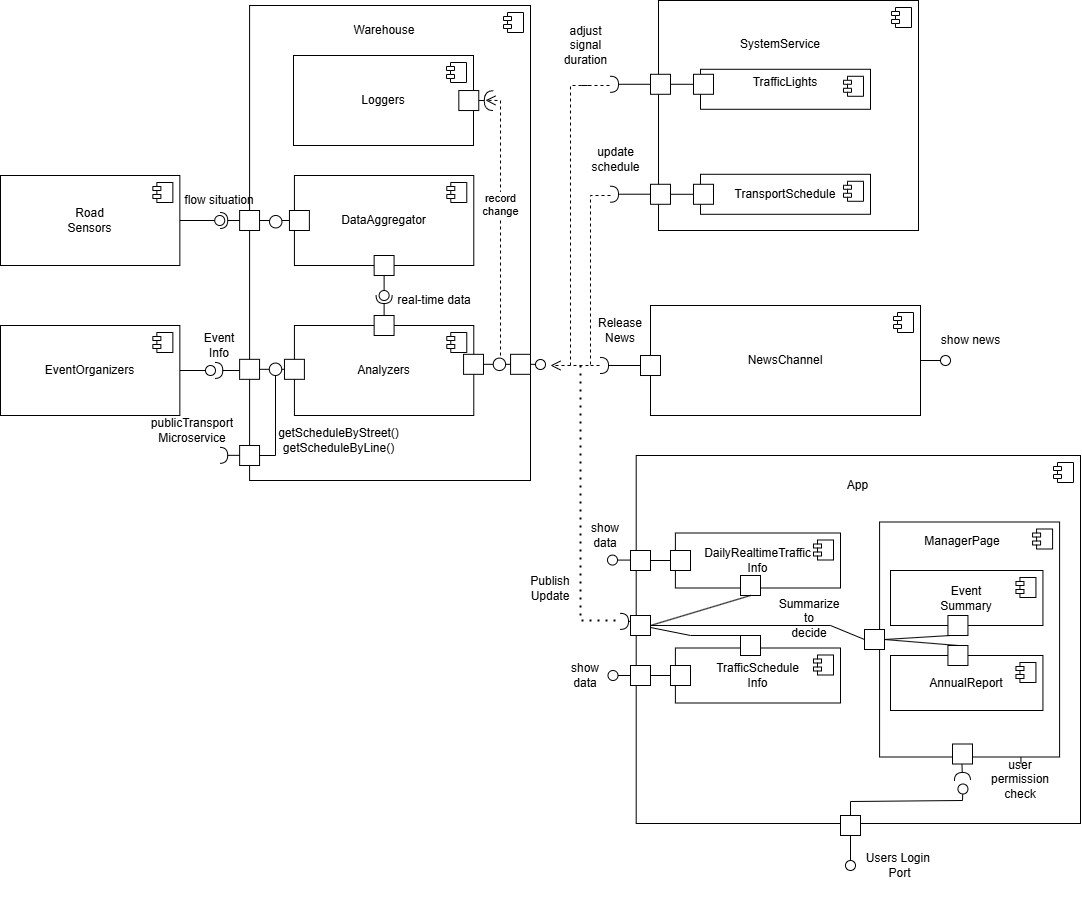
\includegraphics[width=0.95\textwidth]{Images/ComponentDiagram.png}
\end{center}

\paragraph{Component Descriptions:}

\begin{itemize}
    \item \textbf{Road Sensors}: Continuously stream real-time traffic flow data (e.g., congestion levels, vehicle counts) into the system.
    
    \item \textbf{Event Organizers}: Register events that may impact traffic. These inputs are handled by the system through the event dashboard.
    
    \item \textbf{Public Transport Microservice}: An external system providing transport timetables via API calls like \texttt{getScheduleByStreet()} and \texttt{getScheduleByLine()}.
    
    \item \textbf{Data Aggregator}: Collects raw traffic and event data from various sources and prepares it for analysis. Serves as a unified input hub.
    
    \item \textbf{Analyzers}: Responsible for processing different types of data, each dedicated to a specific functionality:

\begin{itemize}
    \item \textbf{Traffic Analyzer}: Handles real-time traffic data to detect congestion and trigger immediate adjustments to traffic lights (Type 1).
    \item \textbf{Pattern Analyzer}: Processes historical traffic data to identify long-term trends and suggest optimizations, such as route or schedule changes (Type 2).
    \item \textbf{Event Analyzer}: Assesses the potential impact of upcoming public events on traffic and transport systems, generating temporary plans and event news.(Type 3).
\end{itemize}

    
    \item \textbf{Loggers}: Record system actions, decisions, and configuration changes for auditing, traceability, and report generation.
    
    \item \textbf{SystemService}: Composed of two internal components:
    \begin{itemize}
        \item \textbf{TrafficLights}: Responsible for adapting signal timings based on analyzer output.
        \item \textbf{TransportSchedule}: Updates public transport schedules in response to congestion or planned events.
    \end{itemize}

    \item \textbf{News Channel}: Receives and displays information about upcoming events.

    \item \textbf{App}: The main interface for users, split into:
    \begin{itemize}
        \item \textbf{DailyRealtimeTrafficInfo}: Displays live traffic data to citizens.
        \item \textbf{TrafficScheduleInfo}: Shows updated public transport schedules.
        \item \textbf{ManagerPage}: Restricted area for traffic managers, with:
        \begin{itemize}
            \item \textbf{Event Summary}: Overview of past and upcoming events.
            \item \textbf{Annual Report}: Summary of yearly system activity and decisions.
        \end{itemize}
    \end{itemize}

    \item \textbf{Users Login Port}: Handles authentication and role-based access control, ensuring the right interface and permissions are applied.
\end{itemize}

Communication between modules is asynchronous and event-driven. This design allows the system to process multiple workflows in parallel (e.g., analyzing traffic while handling events) and maintain high performance under varying load conditions. Each module interacts via well-defined APIs or message-passing interfaces to support scalability and future extensions.

\newpage
\subsection{Sequence Diagrams}

This section presents three key sequence diagrams that illustrate the dynamic interactions between system components, services, and actors. Each sequence diagram corresponds to one of the three functional categories of the system: real-time congestion handling, pattern-based optimization, and event-based traffic planning.

The diagrams highlight:
\begin{itemize}
    \item The main flow of communication between modules.
    \item The triggering actions (e.g., sensor input, event registration).
    \item The system's behavior in processing, logging, and updating external interfaces.
\end{itemize}

\vspace{1em}
\subsubsection*{Type 1 – Adjust Traffic Flow (Real-Time Reaction)}

This diagram describes how the system processes real-time traffic data sent from sensors. The data is aggregated and analyzed, triggering adjustments to traffic light durations. All changes are recorded and traffic summaries are published in the app interface for citizens and managers.

\begin{center}
    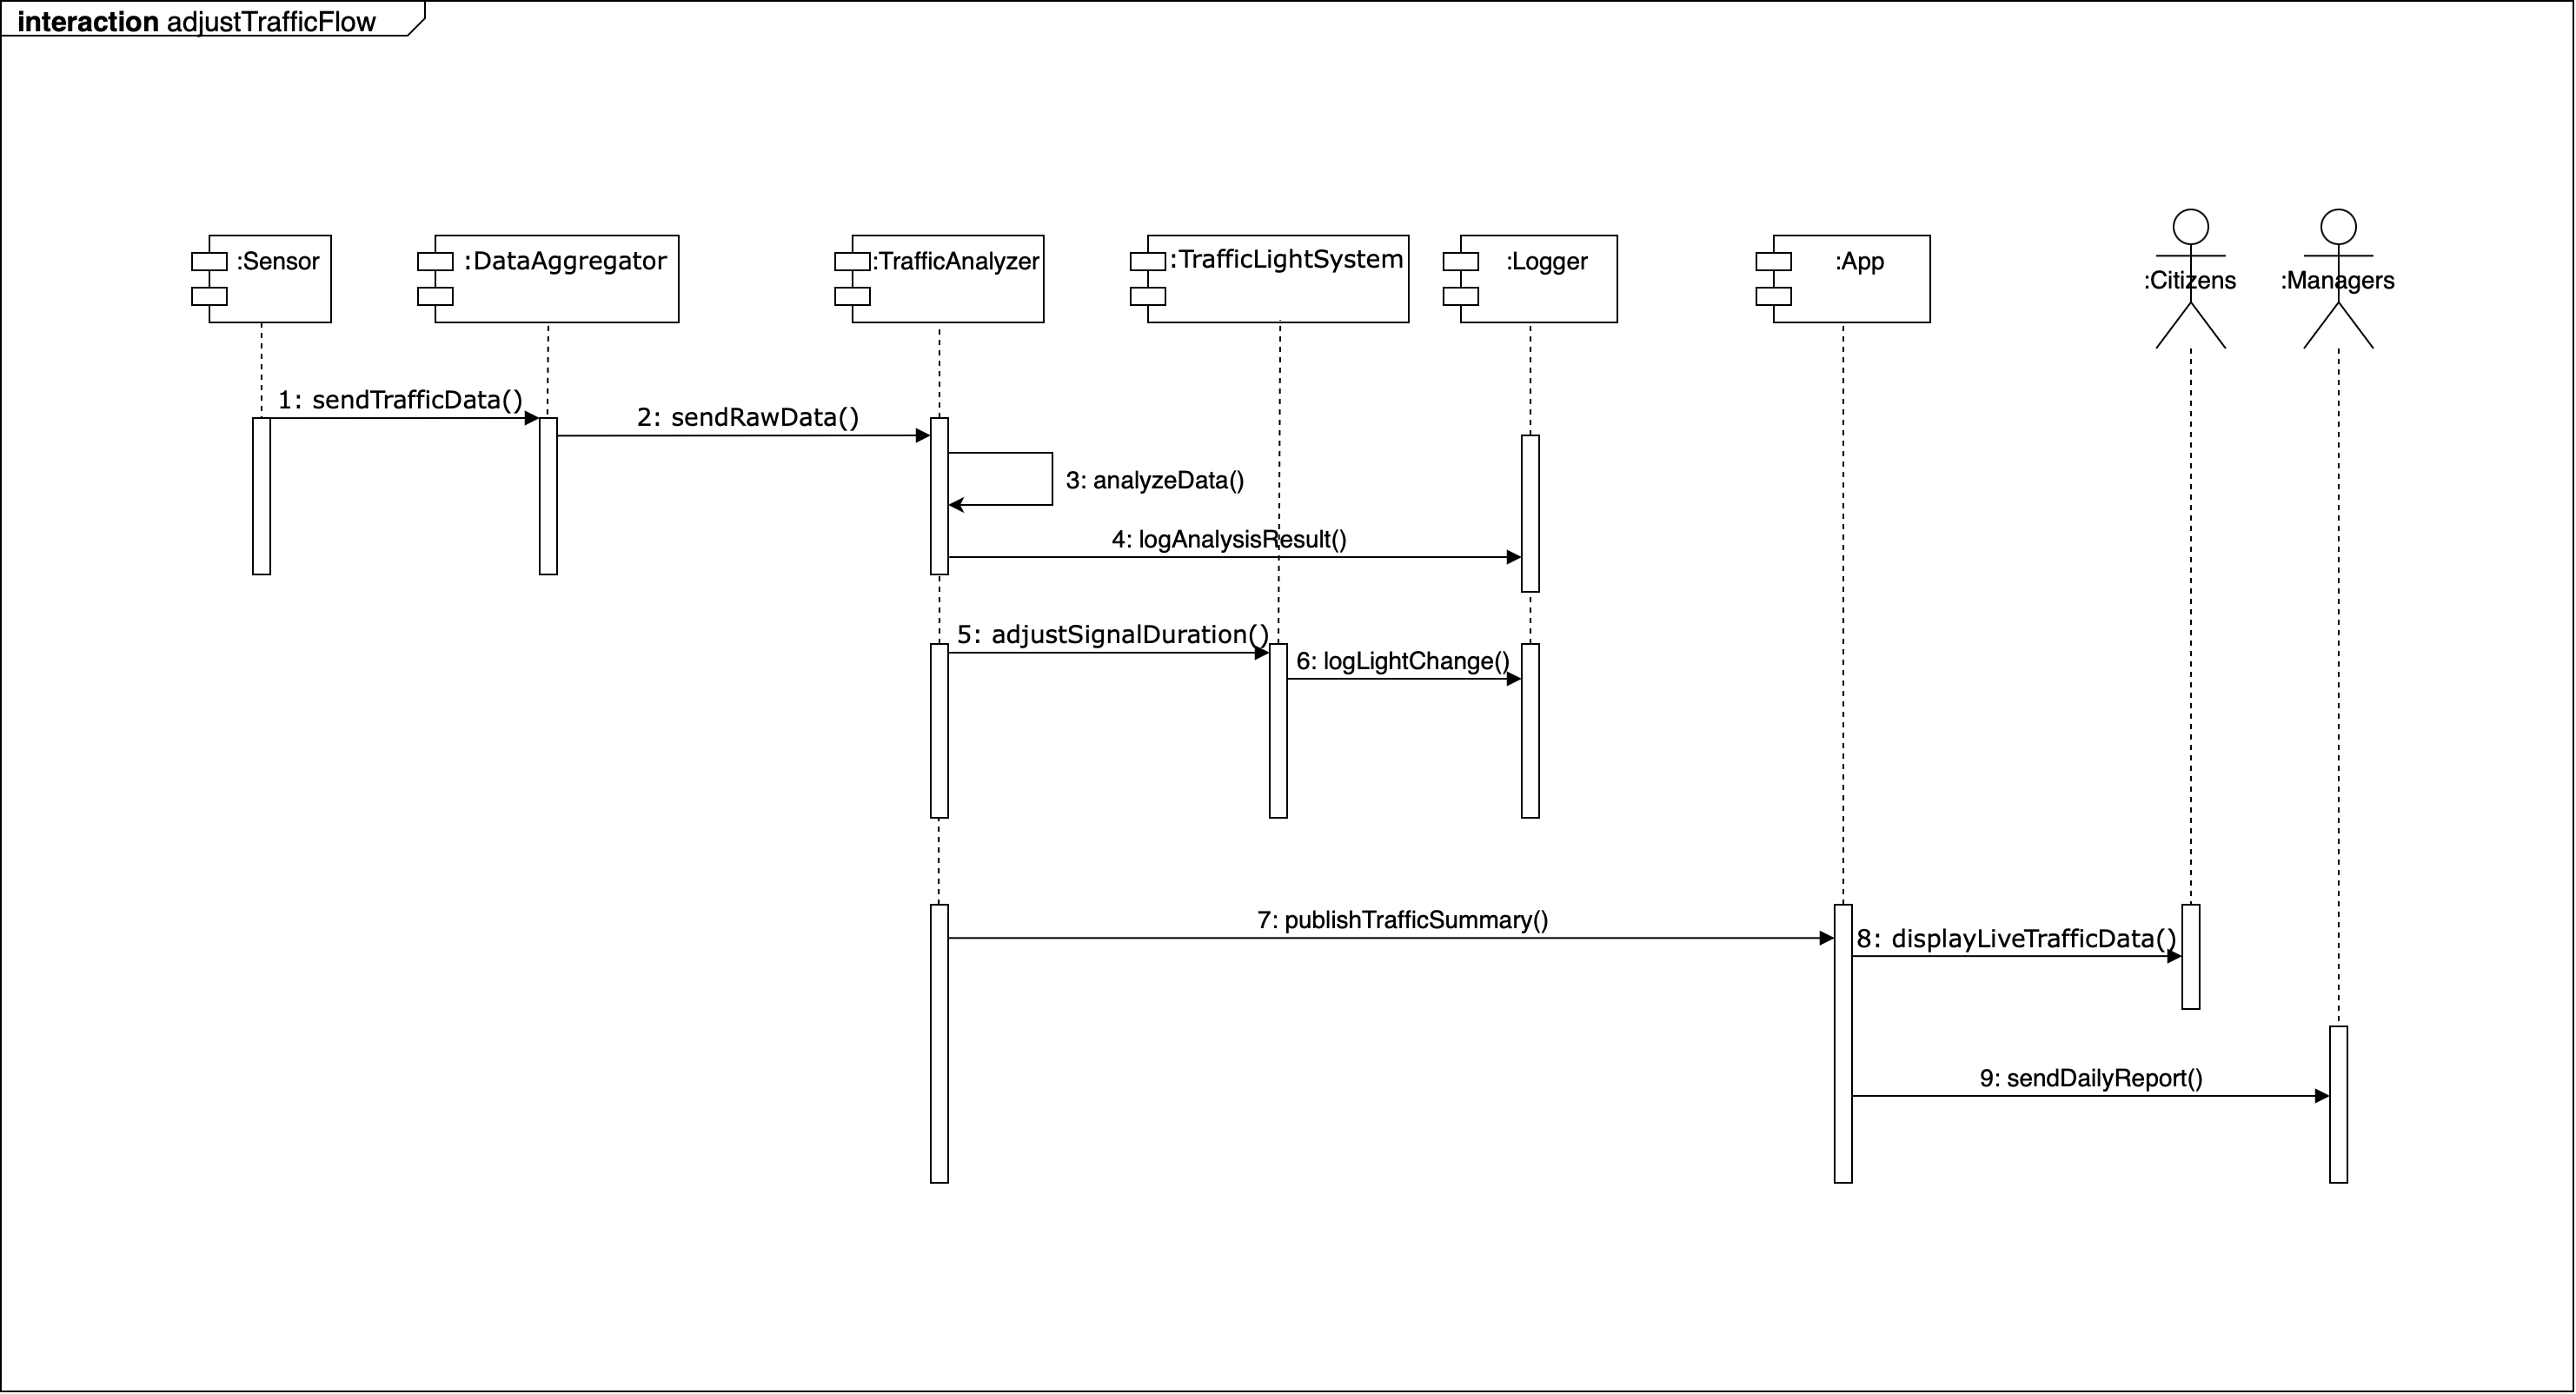
\includegraphics[width=1\textwidth]{Images/t1.sequence.png}
\end{center}





\newpage
\vspace{1em}
\subsubsection*{Type 2 – Suggest Pattern Optimization}

This interaction shows how historical traffic and schedule data are processed by the Pattern Analyzer to generate long-term optimization suggestions. Once approved by traffic managers, updates are made to public transport schedules and traffic light settings. The results are logged and made visible in the annual report.

\begin{center}
    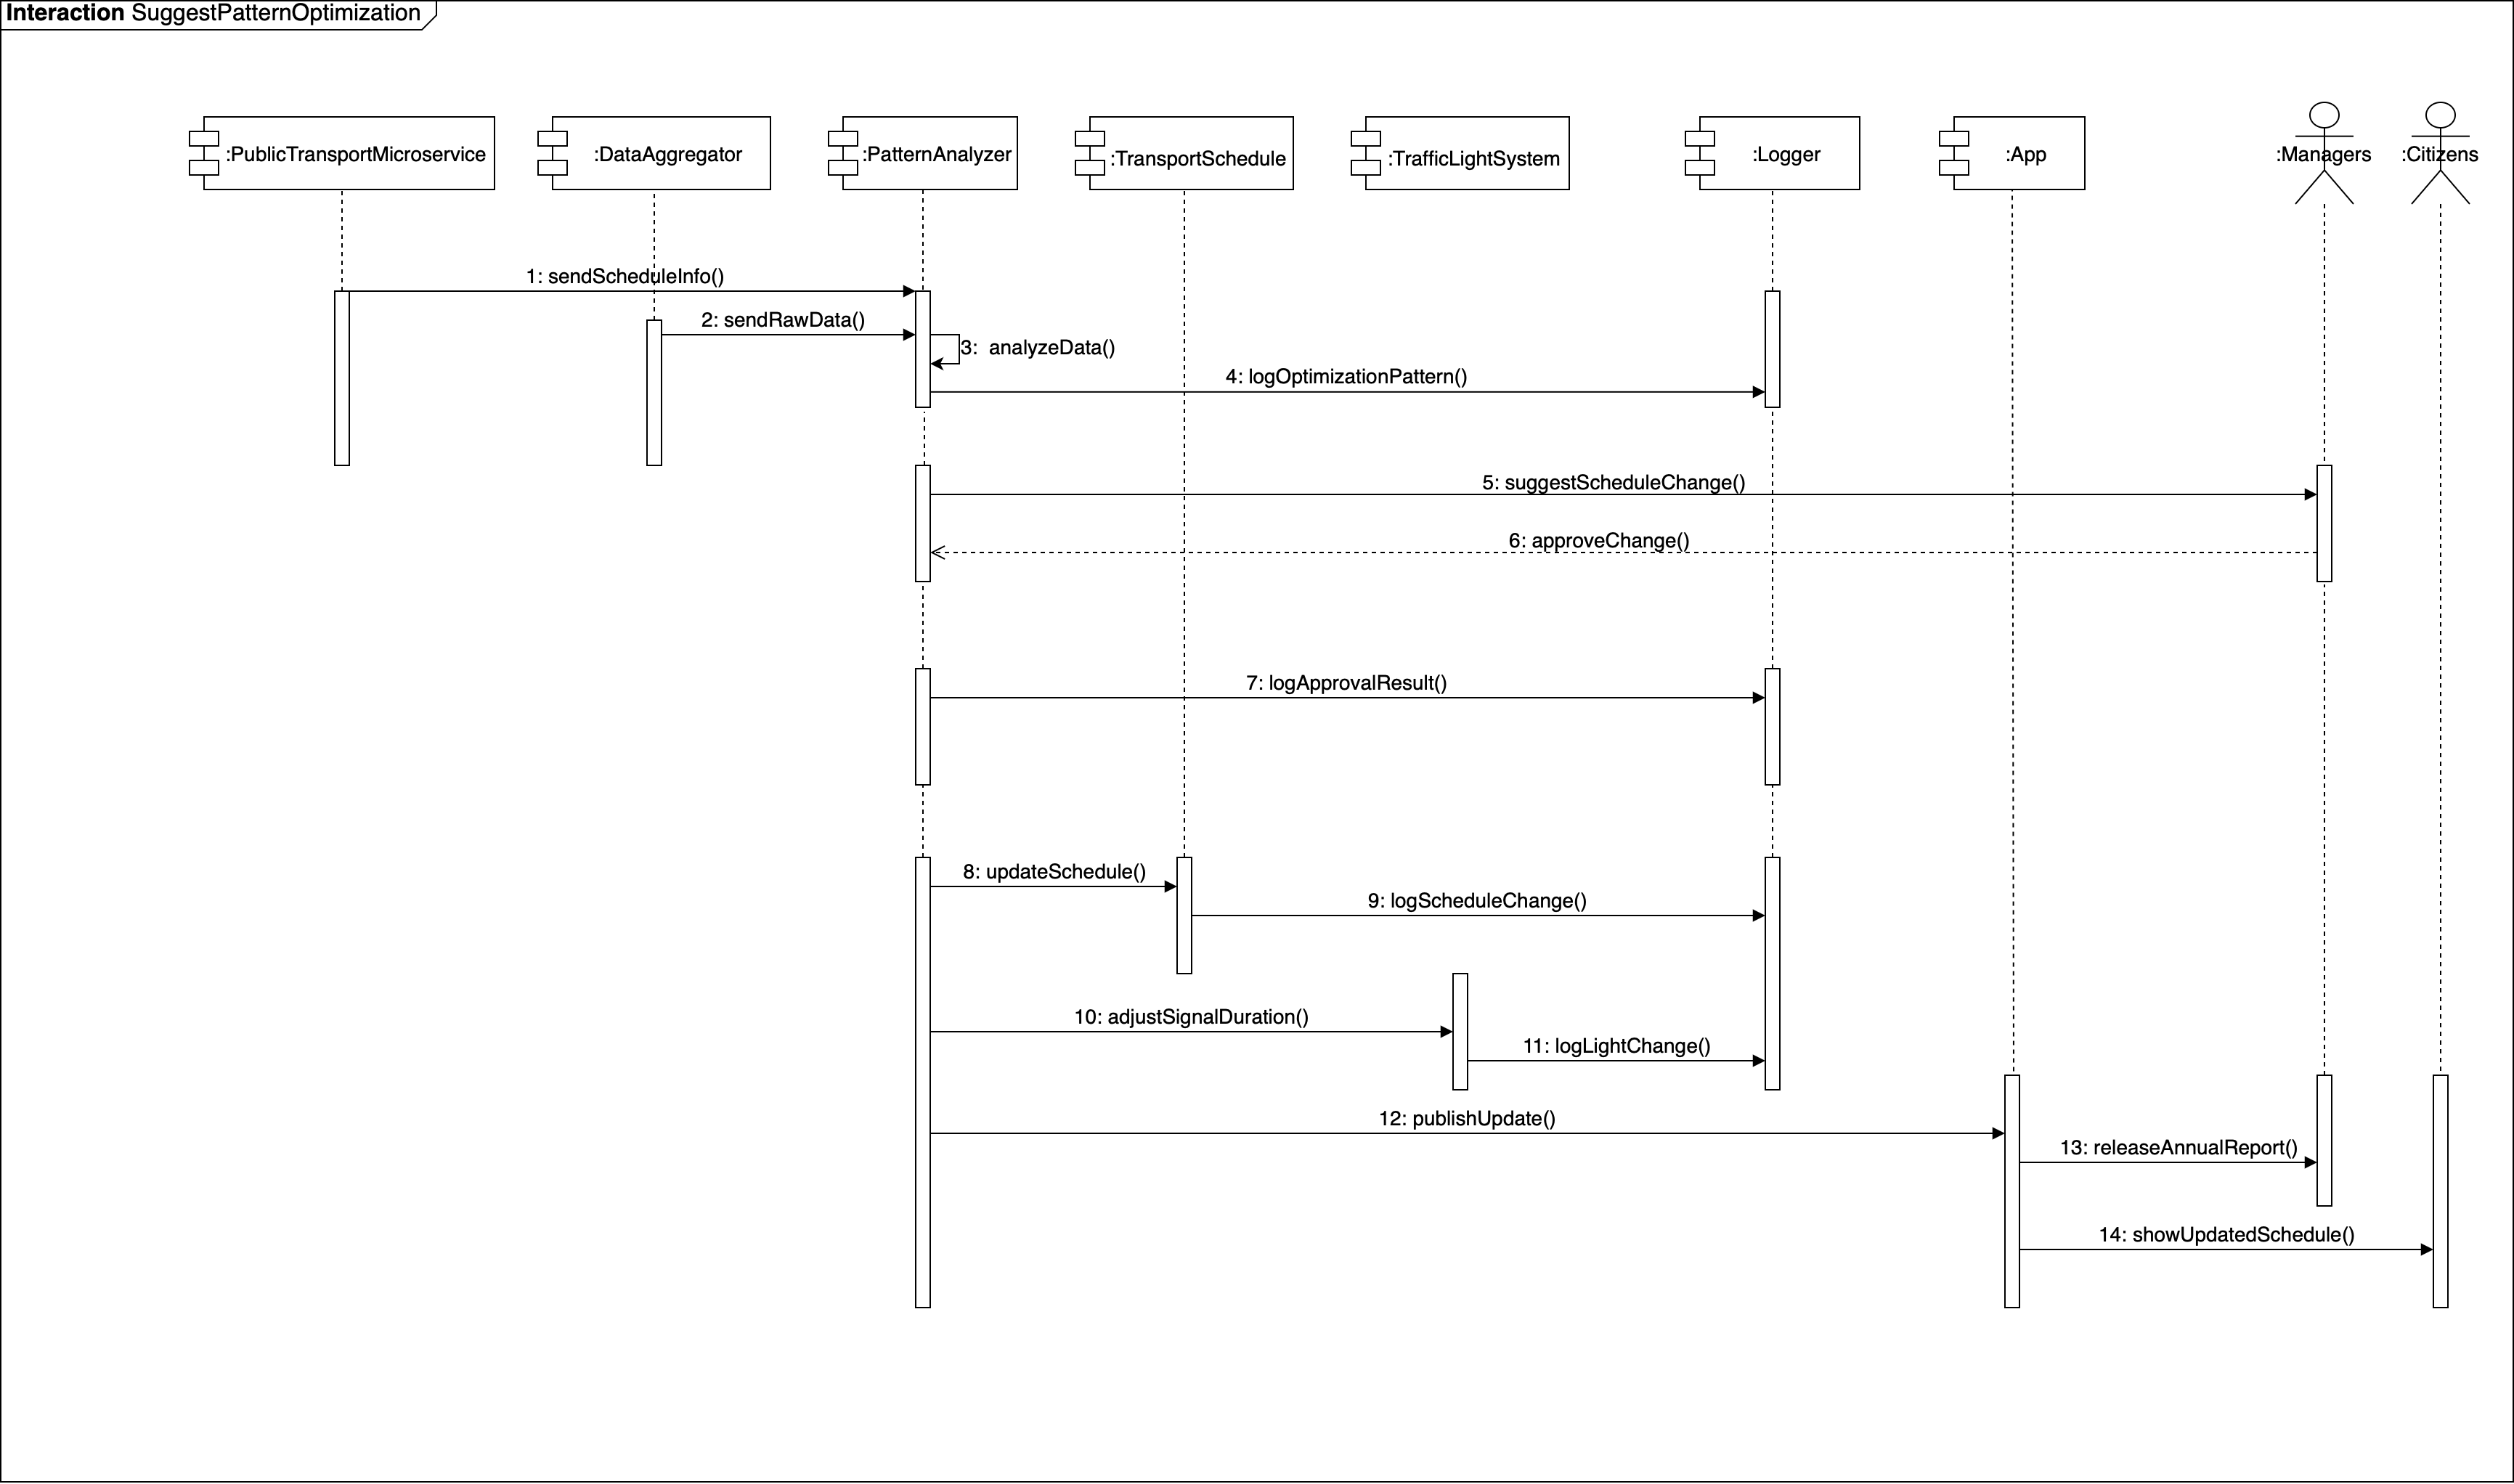
\includegraphics[width=1\textwidth]{Images/t2.sequence.png}
\end{center}

\newpage
\vspace{1em}
\subsubsection*{Type 3 – Change Transport for Event (Event-Based Adaptation)}

This diagram outlines how the system reacts when a new event is registered by an organizer. The Event Analyzer uses current and historical data to suggest temporary traffic and transport changes. Upon approval, configurations are updated, and notifications are sent to citizens through the app and news channels.

\begin{center}
    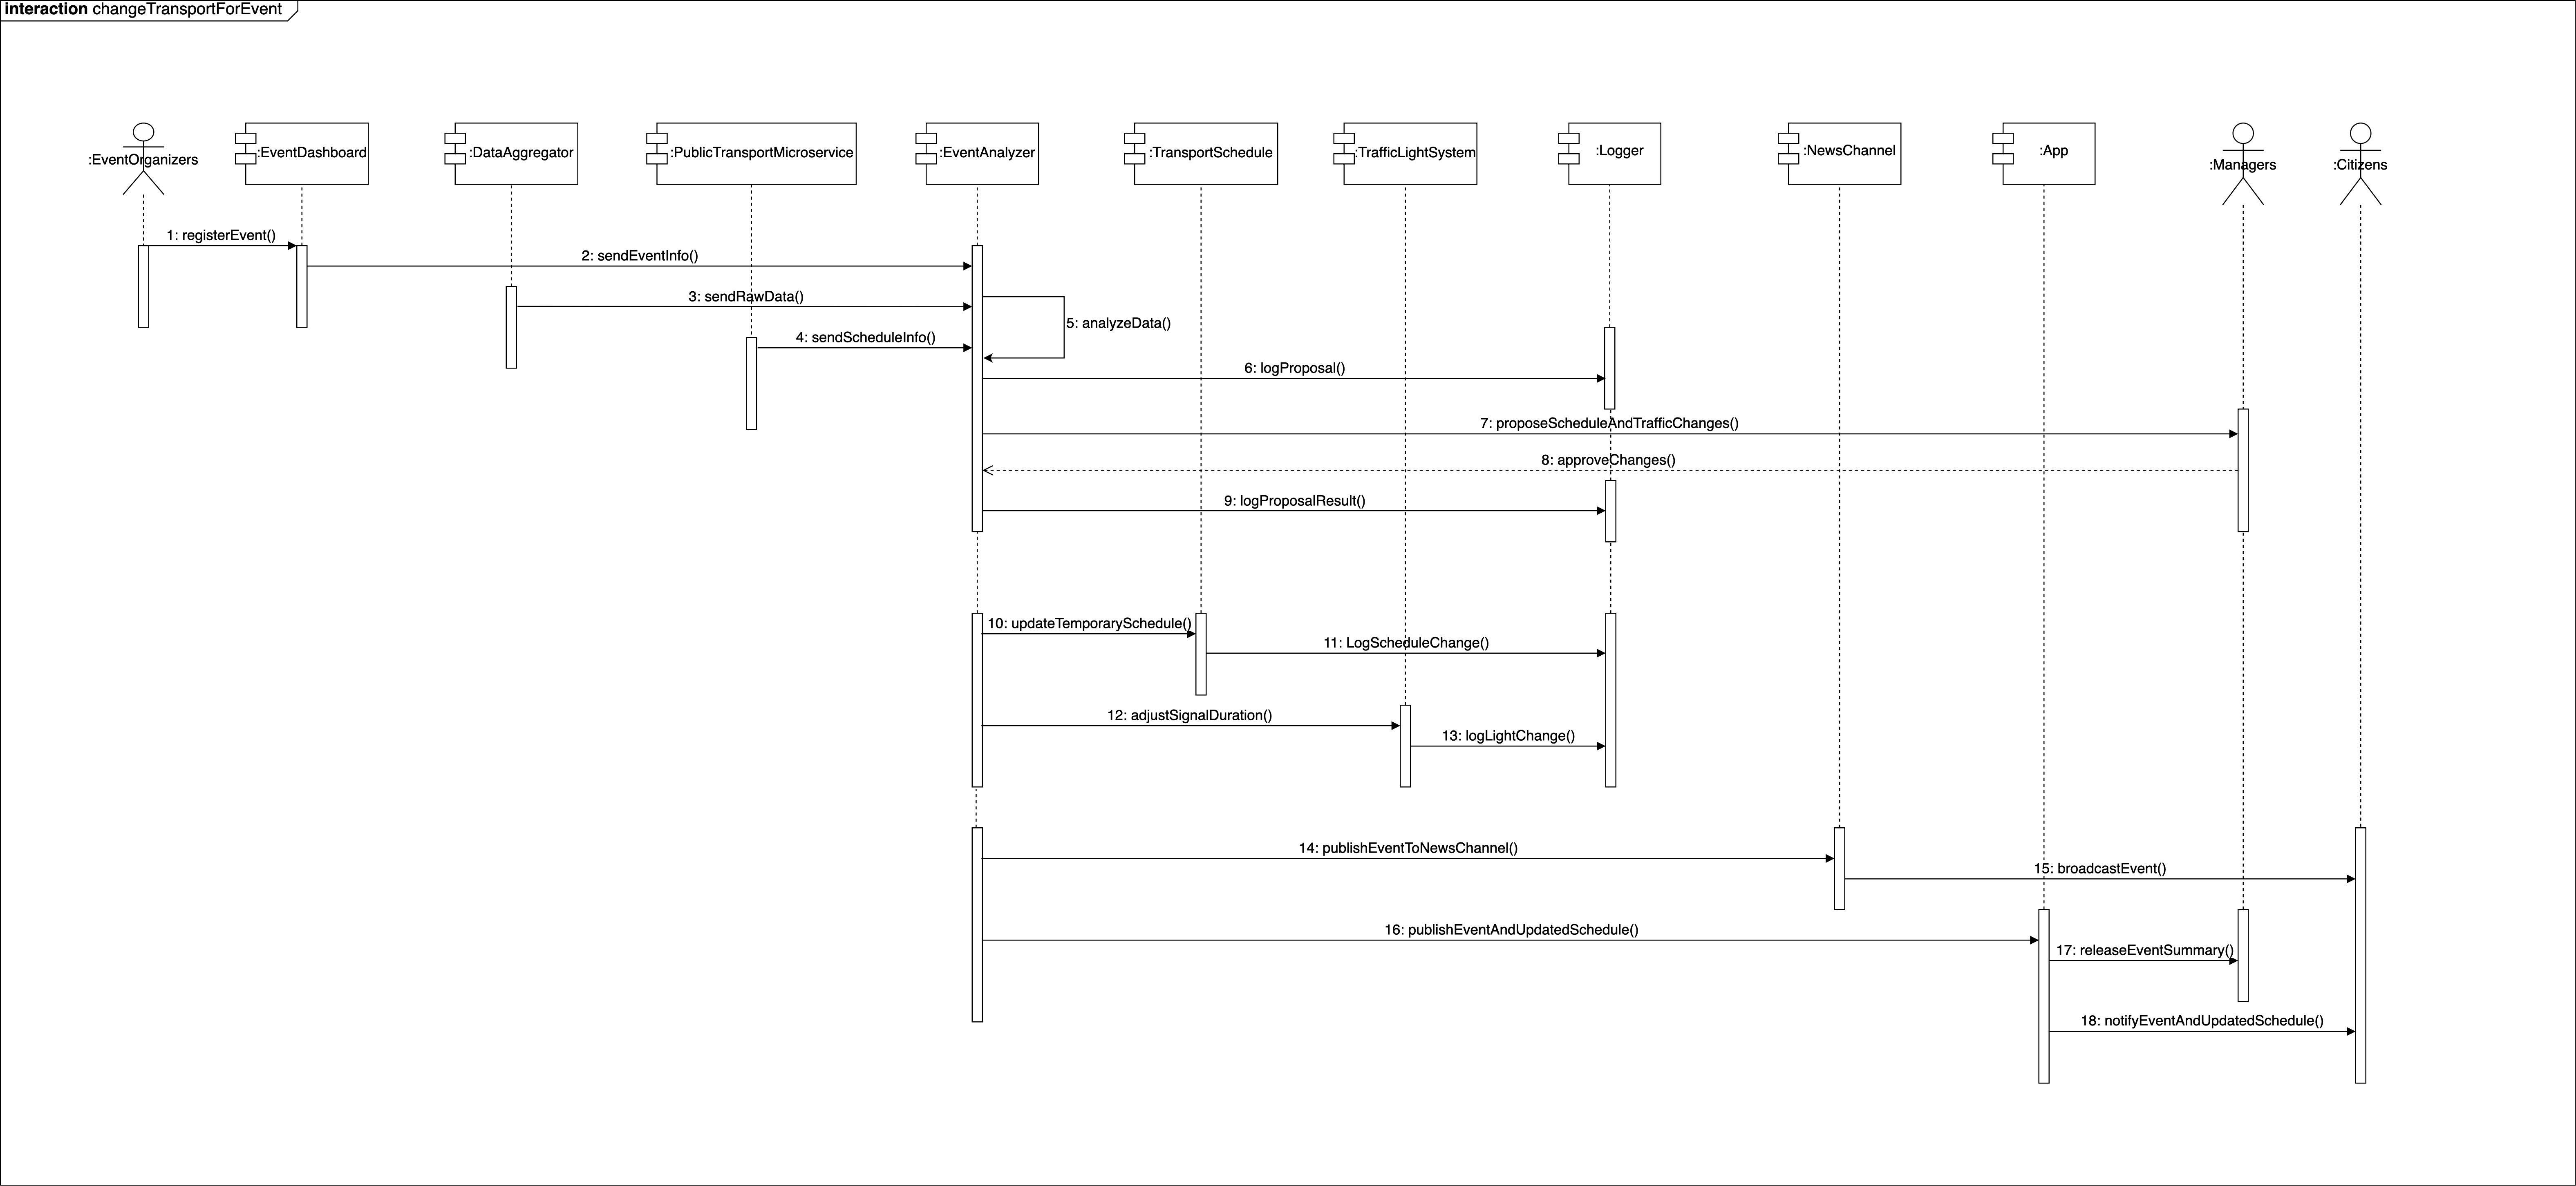
\includegraphics[width=1\textwidth]{Images/t3.sequence.png}
\end{center}




\newpage
\subsection{Critical Points and Design Decisions}

The following architectural and design decisions are directly based on the interactions illustrated in the sequence diagrams. They aim to ensure modularity, reliability, traceability, and scalability of the system:

\begin{itemize}
    \item \textbf{Dedicated Analyzers per Task}: Each main functionality (real-time updates, pattern analysis, and event planning) is handled by a specific analyzer. This separation supports maintainability and allows specialized processing logic for each type of analysis.

    \item \textbf{Centralized Data Aggregation}: All incoming data from external sensors are collected by a shared \texttt{DataAggregator}. This avoids redundancy and ensures consistency in the data used by different system modules.

    \item \textbf{Event-Driven Communication}: The system reacts to incoming data asynchronously. For example, signal adjustments or schedule updates are triggered automatically after analysis, without requiring manual input. This design improves responsiveness and system autonomy.

    \item \textbf{Approval Workflow for Critical Changes}: In Type 2 and Type 3 flows, the system generates suggestions rather than enforcing changes directly. Traffic managers must approve each proposal, ensuring control over modifications to public infrastructure.

    \item \textbf{Separation of Analysis and Execution}: The process of analyzing data and generating suggestions is clearly separated from the components responsible for applying changes. This design reduces the risk of unintended behavior and improves traceability.

    \item \textbf{Comprehensive Logging}: All major actions such as approvals, changes to signal durations, and schedule updates are recorded by the \texttt{Logger}.

    \item \textbf{Role-Specific Interfaces}: The system interface (App) provides different functionalities depending on the user role. Citizens receive real-time updates and routing suggestions, as well as the incoming events, while managers access dashboards to review and check reports.

    \item \textbf{Scalability and Parallel Processing}: The architecture supports multiple independent data flows, as shown in the sequence diagrams. This enables the system to handle concurrent traffic conditions and events without performance degradation.
\end{itemize}


%\newpage
%\section{Dynamic Traffic Light Adjustment (Type 1)}

\subsection*{1. Main Goal}

The main goal of this task is to optimize real-time urban traffic flow by dynamically adjusting traffic light durations based on sensor data. The system detects when a road is experiencing significantly more traffic than crossing roads and modifies green/red light timings accordingly to reduce congestion.

\subsection*{2. Section Goals}

This section focuses on designing a system that automatically monitors traffic patterns through event-based sensors and adjusts traffic lights without human intervention. All actions taken must be logged for traceability, and a daily report is generated to summarize traffic conditions and interventions. The real-time traffic status is also made available to citizens through an application, while only traffic managers have access to daily reports.

\subsection*{3. Requirement Analysis}

\subsubsection*{3.1 Relevant Human and Non-Human Actors}

\textbf{Human Actors:}
\begin{itemize}
    \item Traffic Manager – accesses daily reports summarizing actions taken by the system.
    \item Citizen – views real-time traffic conditions through the application.
\end{itemize}

\textbf{Non-Human Actors:}
\begin{itemize}
    \item Sensor System – provides real-time traffic data through an event-based infrastructure.
    \item Analyzer – processes traffic data and detects imbalances.
    \item Traffic Light System – receives and executes updated timing instructions.
    \item Logger – records each adjustment with metadata for traceability.
    \item Application – provides a user interface for citizens and traffic managers.
\end{itemize}

\subsubsection*{3.2 Use Cases}

\begin{itemize}
    \item Detect high-traffic roads in real time based on sensor data.
    \item Adjust green and red light durations to relieve congestion.
    \item Log each adjustment for traceability.
    \item Generate and provide daily reports for traffic managers.
    \item Display real-time traffic flow data to users via the application.
\end{itemize}

\subsubsection*{3.3 Domain Assumptions}

\begin{enumerate}
    \item Traffic sensors send reliable and periodic data via a message bus.
    \item The Analyzer is able to interpret traffic data within a few seconds.
    \item Traffic Light System supports dynamic configuration of light durations.
    \item Each intersection and road is uniquely identified in the system.
    \item Logger guarantees persistent and tamper-proof logging of actions.
    \item Traffic managers have secure access to daily reports.
    \item Citizens have access to the application interface to monitor real-time traffic.
\end{enumerate}

\subsubsection*{3.4 Requirements}

\paragraph{3.4.1 Functional Requirements}

\begin{itemize}
    \item \textbf{FR1.1:} The system shall receive real-time traffic data from sensors at regular intervals (e.g., every 30 seconds).
    \item \textbf{FR1.2:} The Analyzer shall process incoming data to identify roads with significant congestion.
    \item \textbf{FR1.3:} The system shall dynamically adjust the green/red duration of traffic lights to relieve congestion.
    \item \textbf{FR1.4:} Each light adjustment shall be recorded by the Logger with a timestamp, location, and duration changes.
    \item \textbf{FR1.5:} The system shall generate a daily report summarizing traffic flow and Type 1 actions.
    \item \textbf{FR1.6:} The daily report shall be accessible only by authorized traffic managers.
    \item \textbf{FR1.7:} The real-time traffic conditions shall be viewable by all users via the application.
\end{itemize}

\paragraph{3.4.2 Non-Functional Requirements}

\begin{itemize}
    \item The system shall respond to new sensor data and adjust light durations within 5 seconds.
    \item The system shall be available 24/7 with at least 99\% uptime.
    \item The Logger shall ensure secure, persistent, and traceable storage of all records.
    \item The daily report shall be generated and made available to traffic managers by 00:00 each day.
    \item The system shall be scalable to manage hundreds of intersections across the city.
    \item The application interface shall be responsive and usable on both desktop and mobile devices.
    \item Access to the daily report shall be role-restricted to authorized traffic managers only.
\end{itemize}

%\newpage
%\section{Pattern-Based Optimization (Type 2)}

\subsection*{1. Main Goal}

The goal of this task is to analyze historical traffic patterns to suggest improvements that optimize city traffic flow and public transport efficiency. These include recommendations such as converting streets to one-way directions, adjusting traffic light configurations, or modifying public transport schedules during high-traffic periods.

\subsection*{2. Section Goals}

This section focuses on long-term and recurring improvements based on data trends. The system does not apply these suggestions automatically; instead, it generates structured proposals and submits them to urban traffic managers for approval. All suggestions are logged and used in generating the annual report.

The system reuses aggregated traffic flow data collected and processed by the real-time system developed in Task 1, avoiding redundant analysis of raw sensor input.

\subsection*{3. Requirement Analysis}

\subsubsection*{3.1 Relevant Human and Non-Human Actors}

\textbf{Human Actors:}
\begin{itemize}
    \item Urban Traffic Managers – review and approve or reject the system's suggestions.
    \item Public Transport Schedulers – update transportation schedules based on accepted suggestions.
\end{itemize}

\textbf{Non-Human Actors:}
\begin{itemize}
    \item Public Transport Microservice – provides access to street-based and line-based timetables.
    \item Pattern Analyzer – processes aggregated traffic data and generates optimization suggestions.
    \item Logger – records all suggestions and their status.
    \item Report Generator – compiles annual summaries for all Type 2 suggestions.
    \item Traffic Data Aggregator – provides aggregated data from Task 1.
\end{itemize}

\subsubsection*{3.2 Use Cases}

\begin{itemize}
    \item Identify roads with consistent congestion patterns over time.
    \item Suggest conversion of two-way streets to one-way to improve flow during peak hours.
    \item Recommend modifying traffic light configurations based on frequent directional imbalance.
    \item Suggest updates to public transport schedules to avoid congestion or align with demand.
    \item Recommend increasing service frequency on specific lines during high-usage times.
    \item Log all generated suggestions and whether they are accepted or rejected by managers.
    \item Generate an annual report summarizing all Type 2 suggestions and outcomes.
\end{itemize}

\subsubsection*{3.3 Domain Assumptions}

\begin{enumerate}
    \item Aggregated traffic data is accurate, complete, and accessible from Task 1.
    \item Public transport schedule data is available and regularly updated via microservice.
    \item Managers are responsible for evaluating and approving suggestions.
    \item Urban roads and lights support reconfiguration, including temporary one-way settings.
    \item Public transport lines can be adjusted based on approved scheduling suggestions.
\end{enumerate}

\subsubsection*{3.4 Requirements}

\paragraph{3.4.1 Functional Requirements}

\begin{itemize}
    \item \textbf{FR2.1:} The system shall analyze at least 30 days of historical traffic data to detect patterns of congestion.
    \item \textbf{FR2.2:} The system shall identify roads with frequent directional imbalance and suggest them for one-way configuration during specific time ranges.
    \item \textbf{FR2.3:} The system shall generate suggestions for updating public transport schedules to avoid recurring traffic peaks.
    \item \textbf{FR2.4:} The system shall recommend increased service frequency on heavily loaded transport lines during rush hours.
    \item \textbf{FR2.5:} The system shall present all suggestions to urban traffic managers for review.
    \item \textbf{FR2.6:} The system shall log whether each suggestion was accepted or rejected by the managers.
\end{itemize}

\paragraph{3.4.2 Non-Functional Requirements}

\begin{itemize}
    \item The system shall generate an annual report listing all Type 2 suggestions and their approval status.
    \item The system shall complete analysis of at least 30 days of historical data within 30 minutes.
    \item Each suggestion shall be traceable, with source data references, timestamps, and decision status.
    \item Reports must be exportable in PDF format for archival and communication purposes.
\end{itemize}


%\newpage
%\section{Event-Based Configuration (Type 3)}

\subsection*{1. Main Goal}

The main goal of this task is to collect and analyze information about upcoming events that are likely to attract large crowds (e.g., concerts, sports events, fairs). Based on this data, the system shall generate suggestions for event-specific configurations of traffic lights, road access, and public transport schedules to minimize congestion and ensure smooth urban mobility.

\subsection*{2. Section Goals}

This section focuses on planning ahead for major events by:
\begin{itemize}
    \item Receiving event details through a news feed or input from event organizers.
    \item Estimating traffic impact using historical data gathered by the Task 1 system.
    \item Suggesting changes to mobility configurations in the affected area.
    \item Monitoring live traffic during high-impact events when needed.
    \item Logging suggestions and decisions, and generating a yearly report.
\end{itemize}

\subsection*{3. Requirement Analysis}

\subsubsection*{3.1 Relevant Human and Non-Human Actors}

\textbf{Human Actors:}
\begin{itemize}
    \item Event Organizers – provide event details.
    \item Urban Traffic Managers – review suggestions and activate plans.
    \item Citizens – receive real-time navigation and routing updates via the app.
\end{itemize}

\textbf{Non-Human Actors:}
\begin{itemize}
    \item News Channel(on app) – provides event notifications.
    \item Public Transport Microservice – provides schedule data and supports modifications.
    \item Event Analyzer – evaluates event impact and generates configuration suggestions.
    \item Logger – records all suggestions and manager decisions.
    \item Application – communicates guidance to users and manages interaction with traffic managers.
\end{itemize}

\subsubsection*{3.2 Use Cases}

\begin{itemize}
    \item Receive event data from the News Channel or event organizers.
    \item Analyze affected zones using historical traffic data from Task 1.
    \item Suggest traffic light changes and temporary road restrictions.
    \item Recommend changes to public transport routes or frequency.
    \item Notify citizens through the application interface.
    \item Monitor live traffic and suggest emergency plan activation if needed.
    \item Log all suggestions and decisions for traceability.
    \item Generate a yearly report of all Type 3 proposals and outcomes.
\end{itemize}

\subsubsection*{3.3 Domain Assumptions}

\begin{enumerate}
    \item Event data is provided with sufficient notice and detail.
    \item Daily traffic pattern from Task 2 is accessible and reliable.
    \item Citizens receive and obey guidance via the shared application.
    \item Public transport services support temporary changes.
    \item Emergency mobility plans are pre-defined and can be activated by managers.
\end{enumerate}

\subsubsection*{3.4 Requirements}

\paragraph{3.4.1 Functional Requirements}

\begin{itemize}
    \item \textbf{FR3.1:} The system shall receive event data via the News Channel or organizer interface.
    \item \textbf{FR3.2:} The Event Analyzer shall evaluate event impact using historical traffic data.
    \item \textbf{FR3.3:} The system shall suggest event-specific traffic light configurations and road adjustments based on event plan and real time situation.
    \item \textbf{FR3.4:} The system shall suggest updates to public transport routes or frequencies.
    \item \textbf{FR3.5:} The system shall notify users via the application with event-related guidance.
    \item \textbf{FR3.6:} The system shall monitor live data during events and recommend activating emergency mobility plans if needed.
    \item \textbf{FR3.7:} All suggestions and decisions shall be recorded by the Logger.
    \item \textbf{FR3.8:} The system shall generate an annual report of all Type 3 suggestions and approval outcomes.
\end{itemize}

\paragraph{3.4.2 Non-Functional Requirements}

\begin{itemize}
    \item Suggestions shall be generated within 1 hour of receiving event data.
    \item Event-related updates shall be accessible via mobile and desktop platforms.
    \item The system shall support simultaneous handling of multiple events.
    \item Reports shall be generated App notice format and delivered to traffic managers.
    \item Event-related interfaces shall be restricted to authorized users only.
\end{itemize}



% ----------------------
% ---- DOCUMENT END ----
% ----------------------
\end{document} % Fine documento
